\section{Ejemplos} 
$x^7-x-1$
\begin{figure}[H]
    \centering
    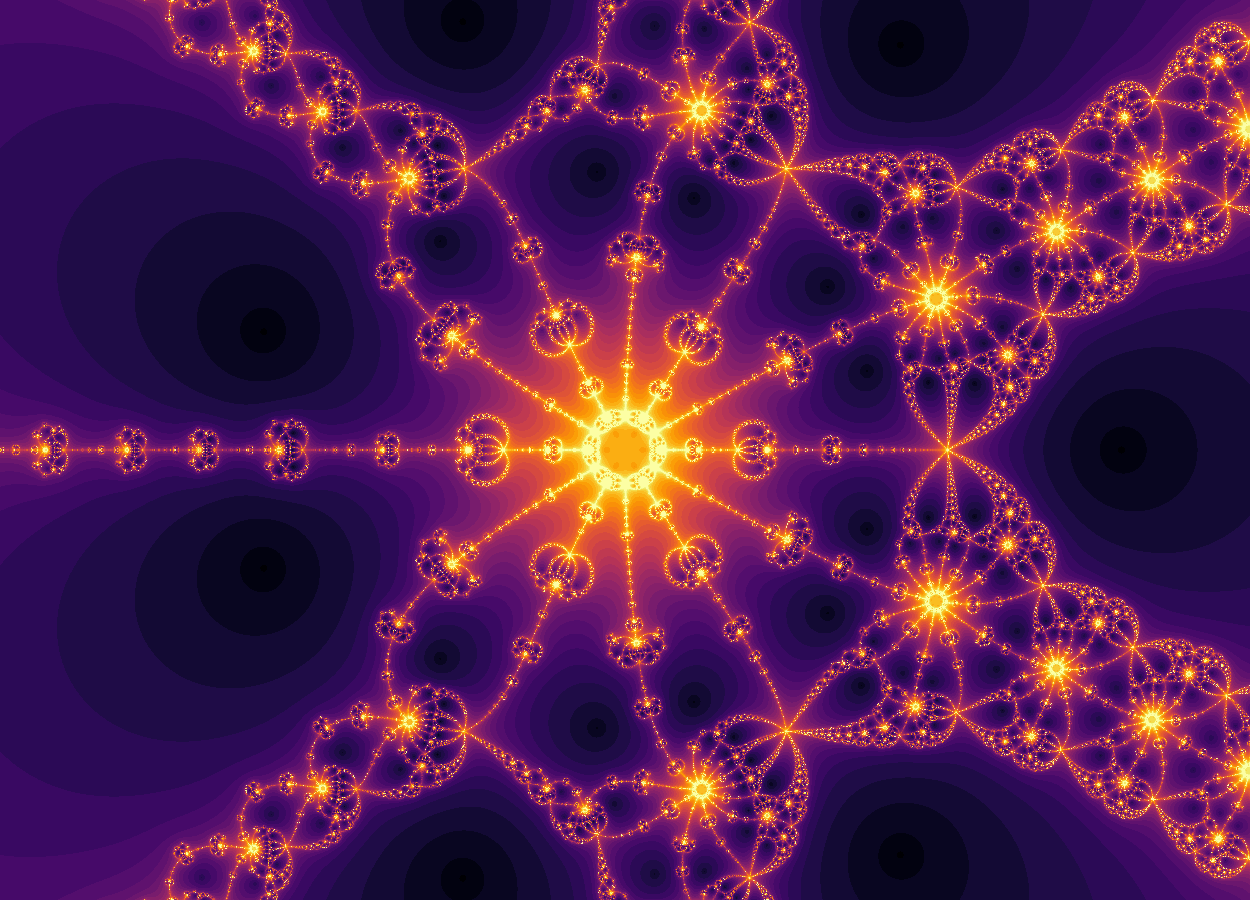
\includegraphics[scale=0.26]{images/ej1.png}
    \caption{Fractal generado por $x^7-x-1$}
    \label{fig:ej_1}
\end{figure}

$x^6-x^3+11$
\begin{figure}[H]
    \centering
    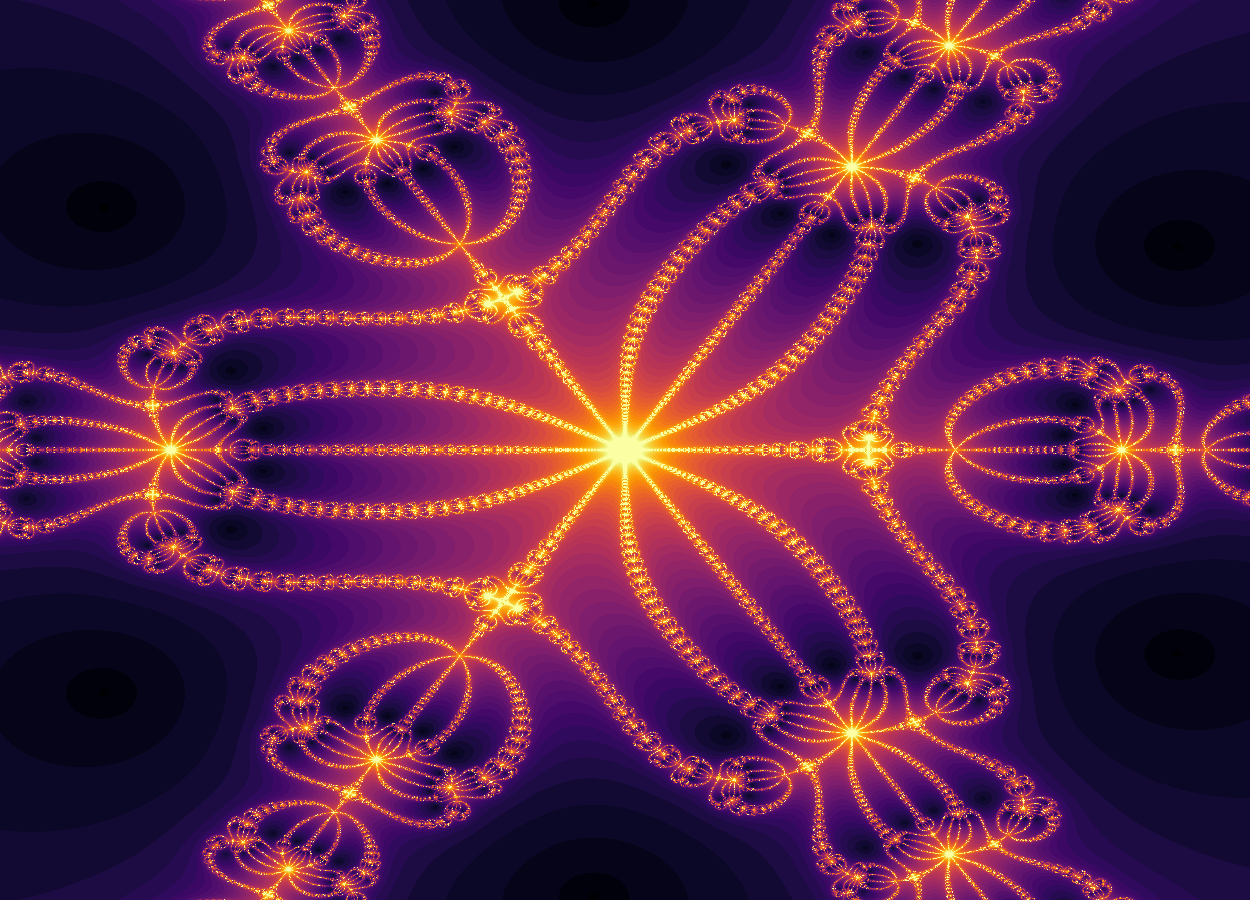
\includegraphics[scale=0.26]{images/ej2.png}
    \caption{Fractal generado por $x^6-x^3+11$}
    \label{fig:ej_2}
\end{figure}

$x^4-x^2-1$
\begin{figure}[H]
    \centering
    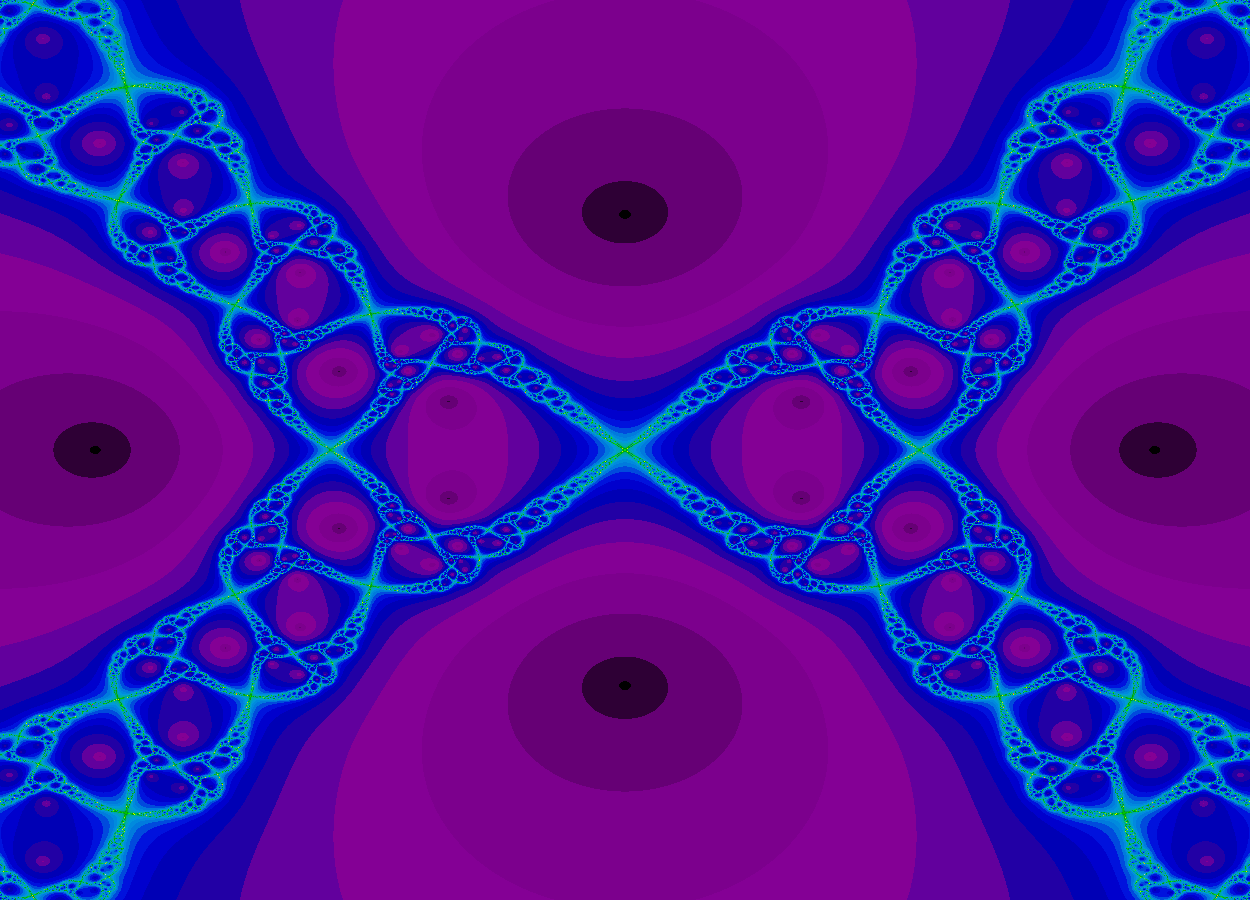
\includegraphics[scale=0.26]{images/ej3.png}
    \caption{Fractal generado por $x^4-x^2-1$}
    \label{fig:ej_3}
\end{figure}

$x^6-3x^2-2x$
\begin{figure}[H]
    \centering
    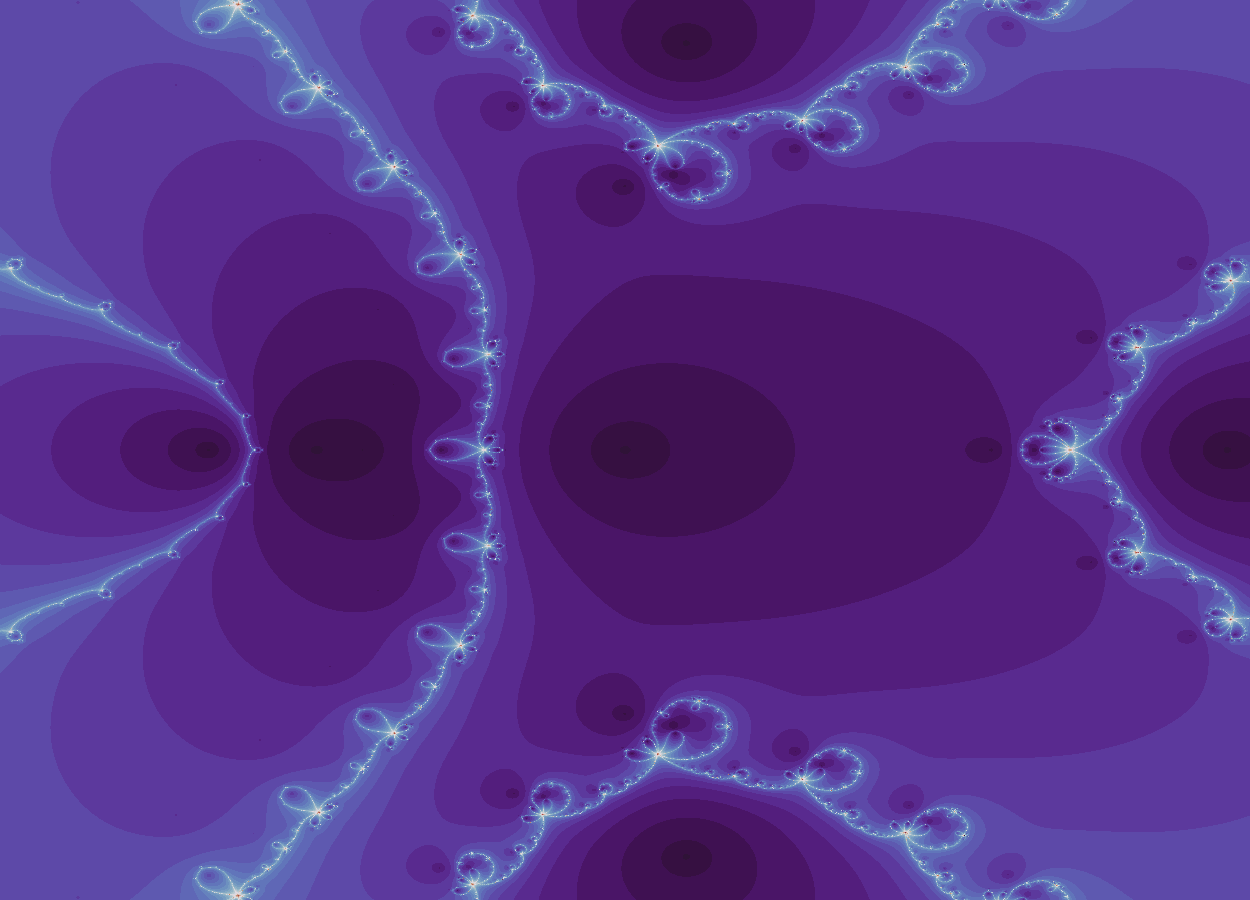
\includegraphics[scale=0.26]{images/ej4.png}
    \caption{Fractal generado por $x^6-3x^2-2x$}
    \label{fig:ej_4}
\end{figure}

$x^7-x^2+1$
\begin{figure}[H]
    \centering
    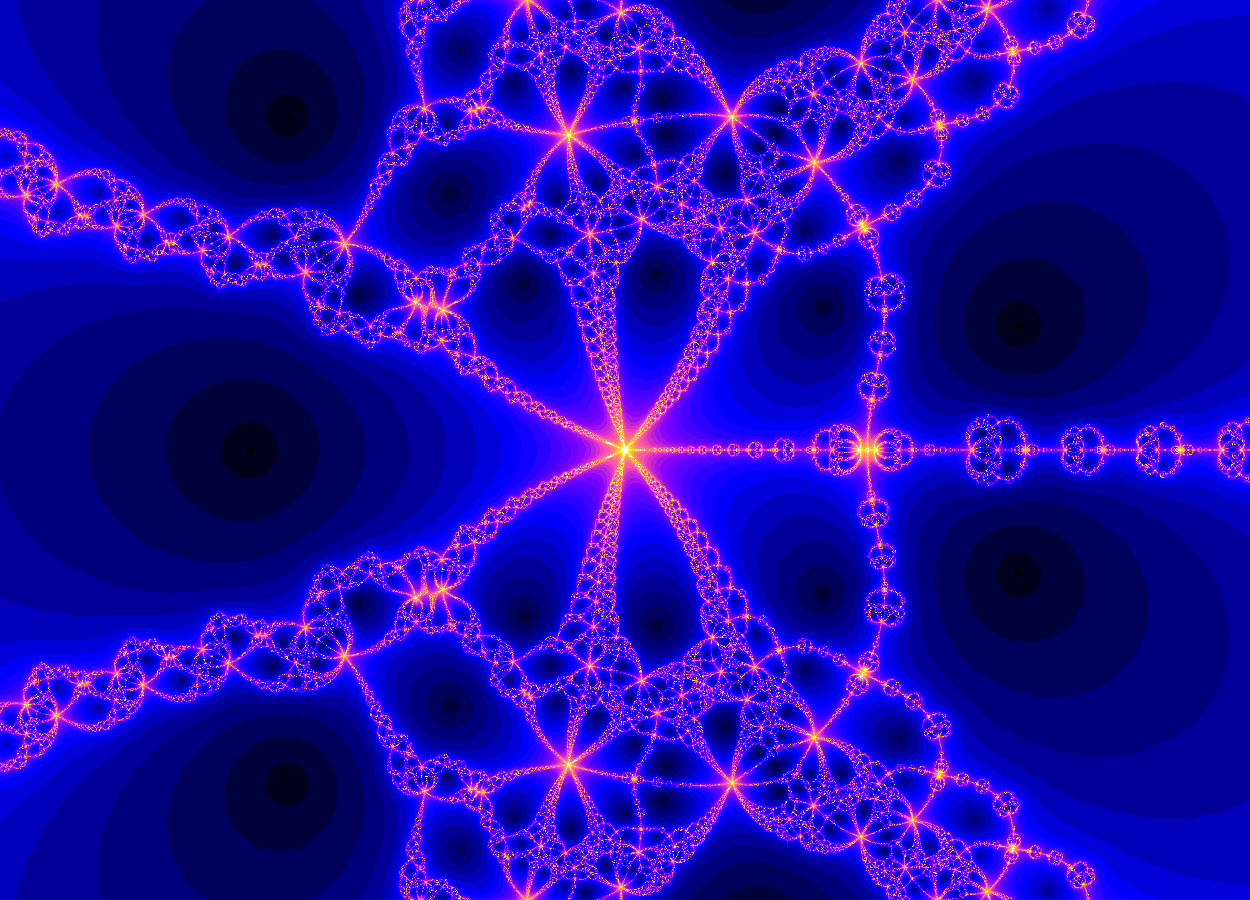
\includegraphics[scale=0.26]{images/ej5.png}
    \caption{Fractal generado por $x^7-x^2+1$}
    \label{fig:ej_5}
\end{figure}

\section{Referencias}

